\section{A faster implementation of the existing balancing algorithm}
\label{sec:packing-code}

The most direct performance result is an optimization of code already in the
reviewed repository. It changes neither the mathematical labeling algorithm
nor its output. The reference is the asymmetric packet's
\texttt{code/balanced\_packing.py} \cite{asymmetric}; a byte-identical copy is
included as \texttt{code/reference\_balanced\_packing.py}. The source already
caches products involving unassigned columns. Our improvement also caches
the row sums used to score every candidate label.

\subsection{Exact conditional expectations}

After the deterministic greedy row labeling, let $Q$ be the number of
labels and let $w_{av}$ be the number of edges from row-label class $a$ to
column vertex $v$. Let $X_{ab}$ be the loads from columns assigned so far.
The reference uses the rational base
\[
 z=1+\frac1{h\max(1,C)},
\]
where $C$ is the maximum column degree and $h\ge2$ is the smoothness
parameter. For each row-label class, define
\[
 F_a=\prod_{v\ \mathrm{unassigned}}\frac{Q-1+z^{w_{av}}}{Q},
 \qquad S_a=\sum_{b=0}^{Q-1}z^{X_{ab}}.
\]
The exact conditional expectation is $\Phi=\sum_a F_aS_a$.
Before assigning column $v$, remove its factor:
\[
 F'_a=F_a\left(\frac{Q-1+z^{w_{av}}}{Q}\right)^{-1}.
\]
All these are ordinary positive rational numbers. They are unrelated to
the nonunit divisions in the two-adic contraction ring.

\begin{proposition}[Cached candidate scores]
\label{prop:scores}
The conditional expectation after assigning $v$ to label $b$ is exactly
\begin{equation}\label{eq:score}
 \Phi_b=\underbrace{\sum_a F'_aS_a}_{B}
       +\sum_a F'_a(z^{w_{av}}-1)z^{X_{ab}}.
\end{equation}
After selecting $b_*$, update
\[
 S_a\leftarrow S_a+(z^{w_{av}}-1)z^{X_{ab_*}},\quad
 z^{X_{ab_*}}\leftarrow z^{X_{ab_*}}z^{w_{av}},\quad
 F_a\leftarrow F'_a.
\]
Every score, its minimizing label with the original tie rule, and the
conditional-expectation certificate are identical to the reference.
\end{proposition}
\begin{proof}
Only cell $(a,b)$ changes when $v$ receives label $b$. Its contribution
to $S_a$ changes from $z^{X_{ab}}$ to $z^{X_{ab}+w_{av}}$.
Subtract the former from the latter and factor the difference to obtain
\eqref{eq:score}. The displayed updates preserve the definitions of $S_a$,
the cell powers, and $F_a$. Induction over columns proves equality with
the reference computation. Since the rational scores are exactly equal,
their ordering, all ties, and the selected labels are equal as well.
\end{proof}

For $N$ column vertices, the reference loops over $Q$ candidate labels,
$Q$ row classes, and $Q$ column classes per assignment. Its candidate-score
phase costs $O(NQ^3)$ rational operations. Formula~\eqref{eq:score} computes
the common base once and uses a $Q$-term correction for each of $Q$ labels,
giving $O(NQ^2)$ rational operations. The additional cell-power cache has
$Q^2$ rational entries. Greedy row assignment, the adjacency scan, and
the shared table of powers $z^0,\ldots,z^M$ remain unchanged. For example,
with $R_0$ input row vertices, a direct overall arithmetic count is
\[
 O(M+R_0N+R_0Q+(N+1)Q^2)
\]
for the new implementation, with $NQ^3+Q^2$ in place of $(N+1)Q^2$ for
the reference's scoring and cell bookkeeping. These are rational-operation counts;
the cost of multiplying long integer numerators and denominators must
still be paid. All operands have the same polynomial bit-length envelope
as in the original method. We do not assert a factor-$Q$ bit-time
speedup on every input.

\subsection{Comparison with the actual reference code}

The verification program compares complete returned objects, including
every exact potential, selected label, cell load, and certificate string.
It passed 840 full-certificate comparisons, covering 9,724 candidate scores;
840 additional comparisons with certificate storage disabled; and 12
invalid-input checks. A normal Python run and an optimized
\texttt{python -O} run give identical verification records. The checks use
explicit exceptions, so optimization does not remove them.

Table~\ref{tab:packing-bench} gives five paired timing trials per instance,
alternating which implementation runs first. Both retain their exact
internal averaging and final-potential checks. Both disable only the
serialization of certificate histories for the timing run. The recorded
JSON includes all trial times and the actual adjacency matrices, permitting
replay without relying on an unspecified input generator.

\begin{table}[htbp]\centering
\caption{Measured packet-labeling times. These are comparisons of the
existing subroutine and its exact replacement, not full SAT timings.}
\label{tab:packing-bench}
\begin{tabular}{@{}rrrrr@{}}\toprule
Rows $\times$ columns & $Q$ & Reference (ms) & Cached (ms) & Ratio\\\midrule
$12\times16$ & 4 & 1.652 & 1.100 & $1.50$\\
$16\times24$ & 8 & 10.974 & 4.111 & $2.67$\\
$20\times32$ & 12 & 39.088 & 9.140 & $4.28$\\
$24\times40$ & 16 & 103.253 & 18.320 & $5.64$\\
$24\times40$ & 24 & 304.464 & 31.833 & $9.56$\\\bottomrule
\end{tabular}
\end{table}

The benchmark is a small, seeded collection on one execution host, using
the recorded Python version and standard-library \texttt{Fraction}
arithmetic. Five repetitions do not establish a cross-machine performance
distribution. The implementation-level saving is nevertheless directly
testable: it performs fewer exact score computations and returns the same
objects as the faster relevant prior implementation. It is suitable for
integration independently of the proposed new asymptotic schedules.

\section{Precision peeling for mode contributions}
\label{sec:peeling}

The source retains a mode tuple $\beta$ when its guaranteed valuation
$V(\beta)=\sum_z w_z\beta_z$ is below the working precision $P$.
It then passes precision $P$ to its child contractions. A further exact
transformation removes those guaranteed powers of two before computing
the contribution. Its correctness does not require a new Cauchy basis,
a particular recursion schedule, or a probabilistic model of the tensor.

\subsection{The algebraic identity}

Use the source's integral coefficient ring
$\mathcal A=\mathcal O[V]/(V^\ell)$, with all congruences interpreted
coordinatewise. Freeze the current tensor entries at their specified
creation-time representatives. Write every targeted mode coefficient as
$c_{xz}=2^{w_z}\bar c_{xz}$, where $\bar c_{xz}\in\mathcal A$.
The affine row factors include local terms $a_x$ and the appropriate signs
from $l_0(t)=1-t$ or $l_1(t)=t$.

\begin{lemma}[Exact coefficient normalization]\label{lem:normalization}
For every multi-index $\beta$,
\begin{equation}\label{eq:normalization}
 [Z^\beta]\prod_x\left(a_x+\sum_zc_{xz}Z_z\right)
 =2^{V(\beta)}[Z^\beta]
       \prod_x\left(a_x+\sum_z\bar c_{xz}Z_z\right).
\end{equation}
\end{lemma}
\begin{proof}
The left polynomial is obtained from the right polynomial by substituting
$Z_z\mapsto2^{w_z}Z_z$. Coefficient comparison gives the identity. It
remains true with cancellations, nilpotent coordinates, and zero terms.
No equality between the valuation of a sum and the minimum valuation of
its summands has been assumed.
\end{proof}

Normalize each packet/group tensor by the contribution of the modes it
targets, leaving source moments unchanged. Let $v_g(\beta)$ be the sum
of target valuations in group $g$. Multilinearity of contraction gives
$Z_{g,\beta}=2^{v_g(\beta)}\bar Z_{g,\beta}$. Every mode has exactly
one target, hence $\sum_gv_g(\beta)=V(\beta)$.

\begin{theorem}[Residual precision]\label{thm:peeling}
For every retained tuple define $Q(\beta)=P-V(\beta)>0$. The recursive
mode identity may be evaluated as
\begin{equation}\label{eq:peeling}
 F(t+\alpha\zeta)\equiv
 \sum_{V(\beta)<P}2^{V(\beta)}
       \prod_g\bigl(\bar Z_{g,\beta}\bmod2^{Q(\beta)}\bigr)
       \pmod {2^P}.
\end{equation}
The normalized children use the same graph and ports. Tuples with
$V(\beta)\ge P$ require no child contraction.
\end{theorem}
\begin{proof}
Apply Lemma~\ref{lem:normalization} separately in every packet and group,
then substitute in the existing exact factorization. Replacing each
normalized factor by its residue modulo $2^Q$ changes its product by a
multiple of $2^Q$. The outside factor $2^V$ makes that error a multiple
of $2^P$. Addition of contributions preserves the congruence.
\end{proof}

\subsection{Division and creation-time representatives}

Two details are essential for a valid implementation. First, to obtain
$\bar c_{xz}$ modulo $2^Q$, compute $c_{xz}$ modulo $2^{Q+w_z}$ and
divide its canonical coordinates by $2^{w_z}$ as ordinary integers.
Alternatively, cancel the known powers in the exact factored formula and
invert only units. Dividing a residue known only modulo $2^Q$ would lose
$w_z$ output bits. For every used mode, $\beta_z>0$ implies $w_z\le V$,
so $Q+w_z\le P$: the original precision already supplies the needed
information. Unused modes can be omitted from that coefficient extraction.

Second, residual precision can decrease along a recursive path. The
source's original implementation assumes increasing precision and freezes
creation-time representatives \cite{upstream}. Therefore the normalized
child must be a newly specified network at precision $Q$. Reduce each
retained parent representative modulo $2^Q$ and freeze the resulting
canonical residue; create normalized packet entries at $Q$ as well.
Later lifting uses these new representatives. It must not return to an
older, larger representative or reevaluate an unfrozen defining formula.

A retained descriptor can carry a precision cap. Further caps flatten
to their minimum, because canonical reductions modulo powers of two
compose. This avoids a growing stack of evaluator wrappers. An older
entry evaluator may still run at its original creation precision before
its result is capped. The theorem does not promise to reduce that cost.

In the cached algorithm, each outer exact-weight array fixes the total
$V$. Consequently $Q=P-V$ is fixed throughout that array, and its entire
triangle multiplication can use the same ring $\mathcal A/(2^Q)$.
Thus peeling is compatible with caching; it does not require adding
quantities from different residue rings in a single matrix product.

\subsection{What arithmetic work can be saved}

Let $N(t)$ count feasible tuples with $V<t$; additional fixed support or
degree constraints may be included. The total precision charge for one
linear-in-precision operation per contribution has the exact identity
\begin{equation}\label{eq:layercake}
 \sum_{V(\beta)<P}(P-V(\beta))=\sum_{t=1}^P N(t)
 \le P N(P).
\end{equation}
To prove it, write each positive integer $P-V$ as a sum of $P-V$ ones
and exchange the two finite sums. More generally, for nondecreasing $f$
with $f(0)=0$,
\begin{equation}\label{eq:generalcharge}
 \sum_{V(\beta)<P} f(P-V(\beta))
 =\sum_{q=1}^P\bigl(f(q)-f(q-1)\bigr)N(P-q+1).
\end{equation}
These are operation-charge identities, not wall-clock predictions.

There is also a useful certified upper estimate. Put
$\mathcal Z(\theta)=\prod_z(1-e^{-\theta w_z})^{-1}$ for positive weights.
For any $\alpha>0$ and $\theta>0$,
\begin{equation}\label{eq:tilted-work}
 \sum_{V(\beta)<P}(P-V(\beta))^\alpha
 \le\left(\frac{\alpha}{e\theta}\right)^\alpha
       e^{\theta P}\mathcal Z(\theta).
\end{equation}
Indeed $q^\alpha e^{-\theta q}\le(\alpha/(e\theta))^\alpha$ for $q>0$,
and extending the remaining sum to all tuples gives $\mathcal Z$.
For the same tilted counting certificate, full precision contributes
$P^\alpha e^{\theta P}\mathcal Z(\theta)$. The ratio of these two upper
certificates is $(\alpha/(e\theta P))^\alpha$.
At the contraction saddle, $\theta P\asymp M/\sqrt u$, giving a
polynomial prefactor saving in this specified arithmetic model.
This is not a ratio of actual runtimes, nor a proof that all oracle work
scales with residual precision.

An exact dynamic program for four colored families of weights
$5+4j-2s_2(j)$ at $P=1024$ gives mean residual precision about $25.04$
bits and linear precision-charge ratio $0.02445$. This is an abstract
infinite-family partition inventory truncated by the budget, not an
assertion that one particular finite packet has that distribution.
Finite packet lengths and active valuation levels must still be supplied
when using the model for a concrete network.

Peeling leaves the number of mode tuples unchanged. Moreover the existing
global schedules make the next Hermite loss dominate the inherited
precision. The present argument therefore does not decrease the leading
$s/\sqrt{\log s}$ entropy term by itself. Its useful scope is arithmetic
that is actually moved to the smaller residue ring.

\subsection{Executable evidence}

The self-contained prototype checks 544 randomized cyclic tensor
contractions, including 120 terms vanishing by valuation. It also compares
18 mode contractions of actual permissible Cauchy subblocks with direct
original-kernel sums at precisions from 8 through 80, rejects four invalid
normalizations, and runs 1,601 canonical-cap regressions. Normal and
optimized Python runs agree. The actual-domain test uses an independent
exact rational elimination to reconstruct the relevant Cauchy block,
rather than importing the prior feature implementation.

Table~\ref{tab:peeling-bench} measures a separate arithmetic kernel:
the cyclic contraction of five dense $12\times12$ matrices, with input
precision $P=2048$ bits and controlled total divisibility $V$.
Both methods receive the same frozen canonical inputs. The peeled time
includes validation and normalization; input generation is excluded from
both timings. Seven paired trials alternate execution order.

\begin{table}[htbp]\centering
\caption{Synthetic cyclic-contraction speed ratios, including normalization.
These quantify an arithmetic kernel, not a complete SAT algorithm.}
\label{tab:peeling-bench}
\begin{tabular}{@{}rrr@{}}\toprule
Removed bits $V$ & Residual precision $Q$ & Full/peeled median time\\\midrule
0 & 2048 & $0.99$\\
512 & 1536 & $1.63$\\
1024 & 1024 & $3.11$\\
1536 & 512 & $6.63$\\
1792 & 256 & $9.48$\\
1984 & 64 & $14.34$\\\bottomrule
\end{tabular}
\end{table}

The zero-valuation row records the small overhead when there is no
precision to remove. The other rows show why the transformation can be
useful, while leaving open the frequency and cost share of such operations
in a complete implementation. All trial times, seeds, dimensions, and
environment metadata are retained in the accompanying JSON.

\begin{figure}[htbp]\centering
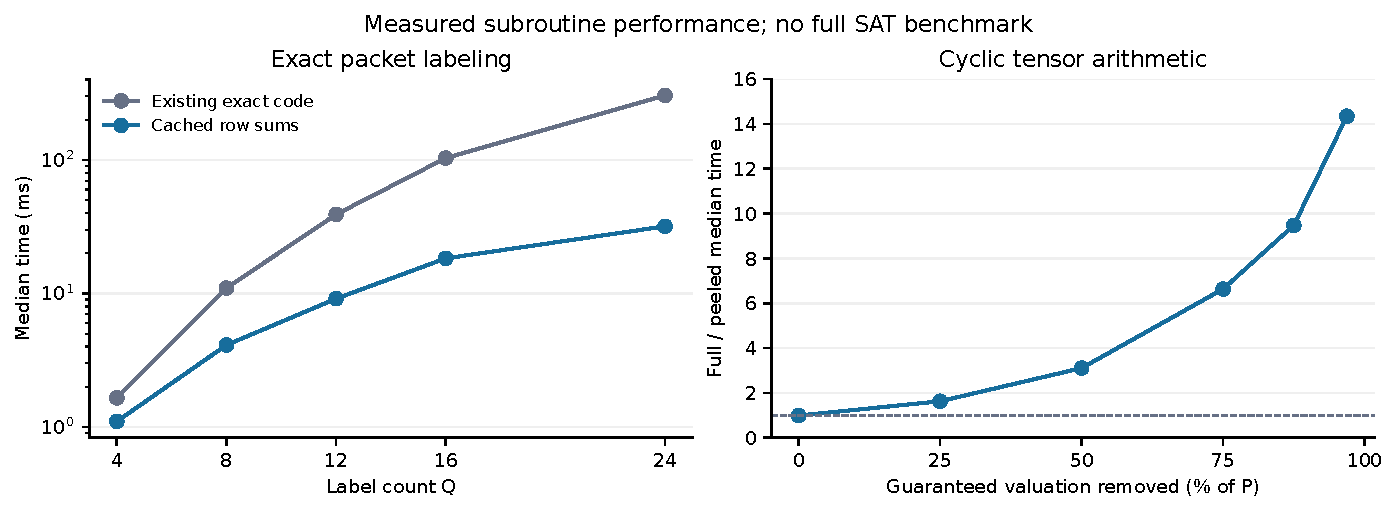
\includegraphics[width=\textwidth]{figures/kernel_benchmarks.pdf}
\caption{Two distinct measured improvements. Left: the existing exact
labeling code versus its cache-preserving replacement. Right: full-precision
versus normalized cyclic matrix contraction. The panels have different
workloads and should not be multiplied into a predicted SAT speedup.}
\label{fig:benchmarks}
\end{figure}
